\section{Hardware}

I dette afsnit vises domain model og tilhørende beskrivelse.
Domain modellen bruges som et bindeled mellem kravspecifikationen og systemarkitekturen.  

I det følgende afsnit beskrives systemet hardware vha. SysML diagrammer. 
Indledningsvis bruges bdd'er til at identificere og beskrive systemets blokke. Senere i afsnittet vises blokkenes interne og eksterne forbindelser med ibd'er.

\subsection{Block definition diagram}
I det overordnede bdd nedenfor vises hvilke blokke systemet består af samt hvilke parts blokkene har. På figur \ref{fig:bdd_overordnet} ses det at systemet helt overordnet set kun består af de to blokke - \textit{Webapplication} og \textit{Drone}. 

\begin{figure}[H]
\centering
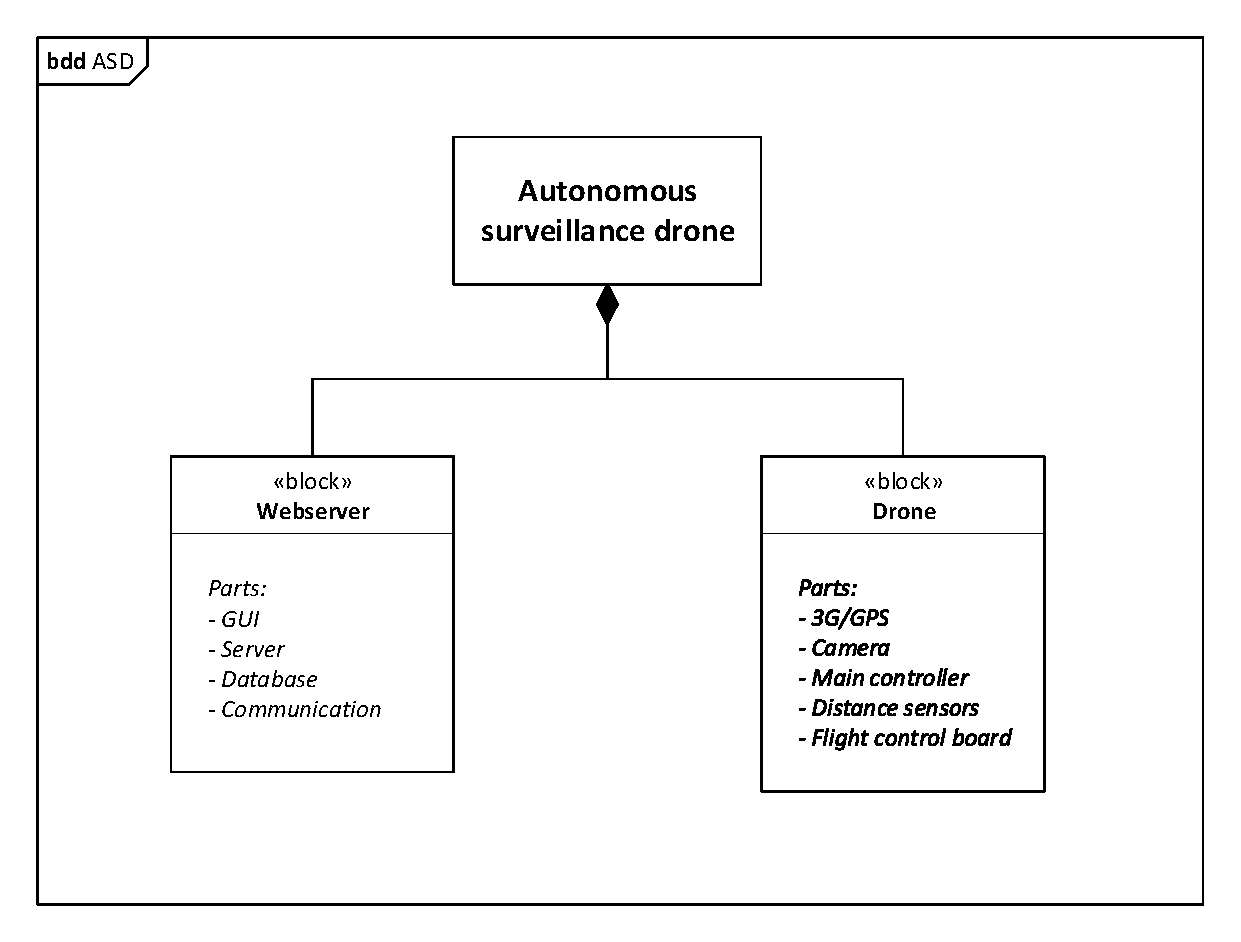
\includegraphics[width=1\textwidth]{Billeder/BDD/bdd_overordnet.pdf}
\caption{Overordnet bdd}
\label{fig:bdd_overordnet}
\end{figure}

\newpage
\subsubsection{Udvidet - Block definition diagram}
Figur \ref{fig:bdd_drone} går mere i dybden med drone blokken, her vises de blokke dronen er bygget af.

\begin{figure}[H]
\centering
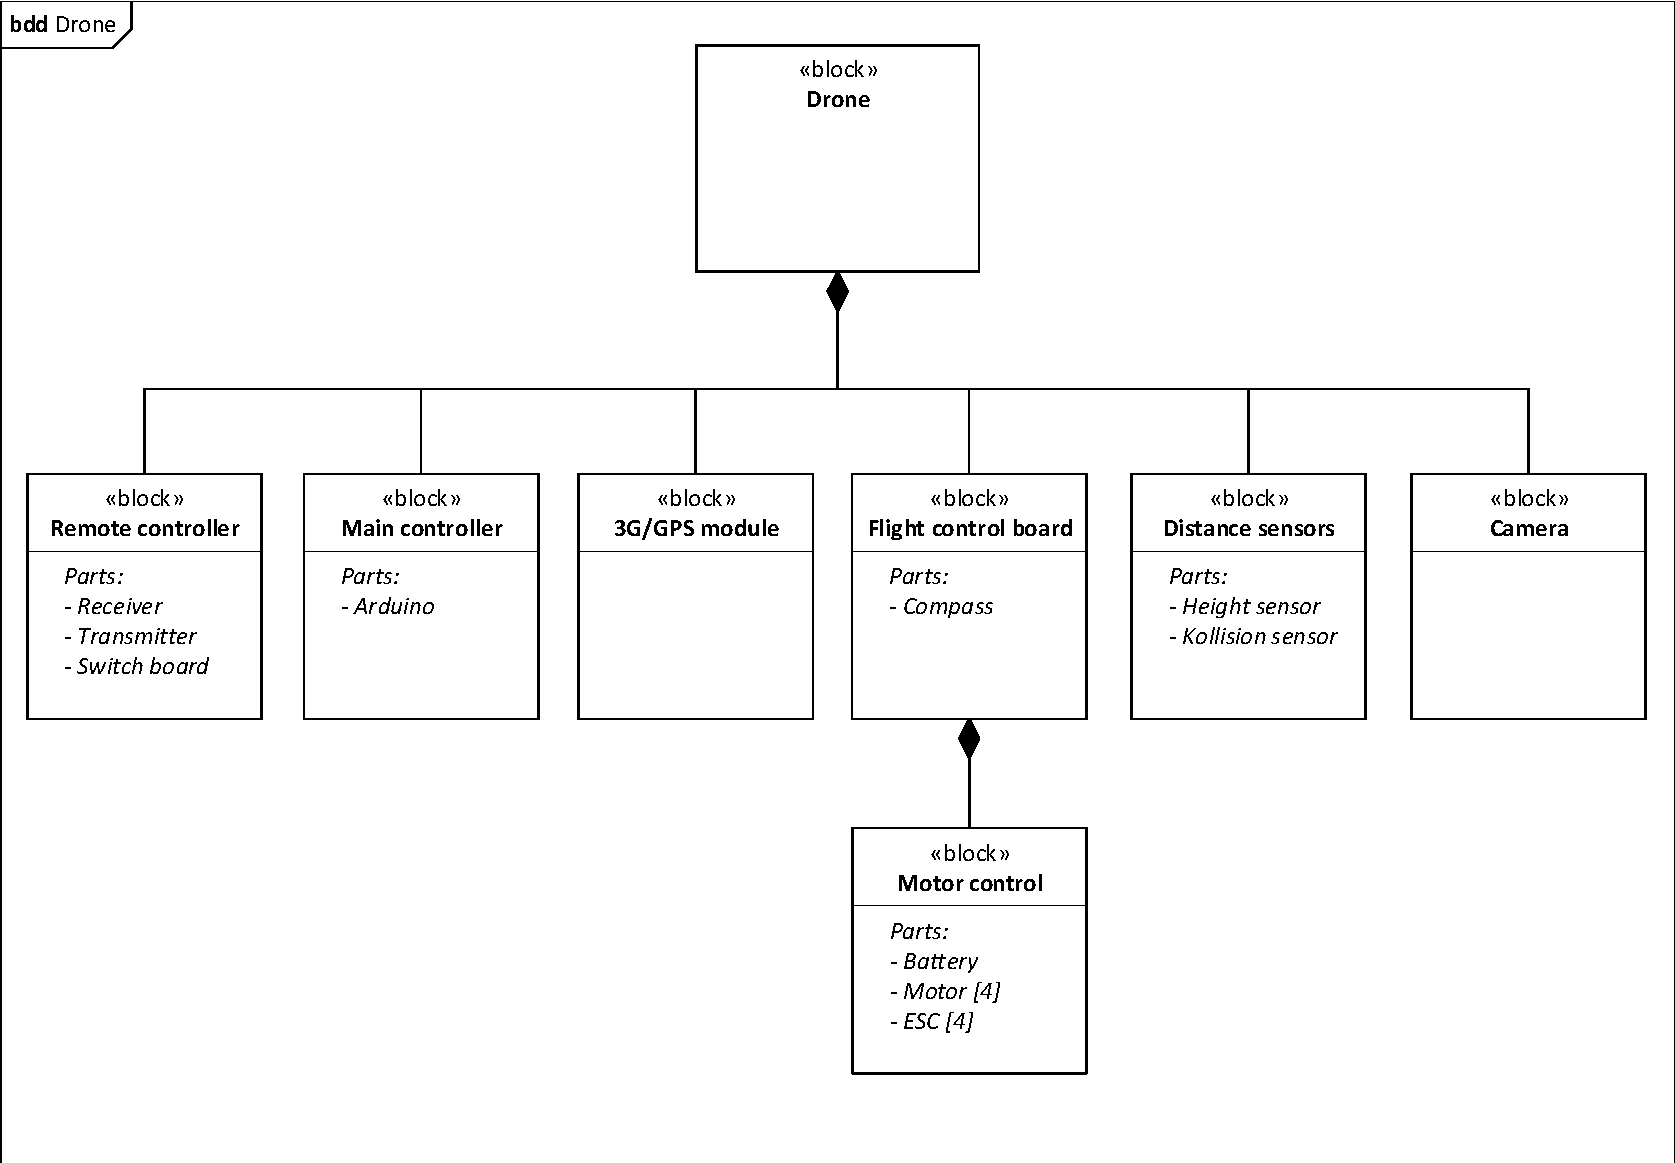
\includegraphics[width=1\textwidth]{Billeder/BDD/bdd_drone.pdf}
\caption{Drone - bdd}
\label{fig:bdd_drone}
\end{figure}


\subsubsection{Blokbeskrivelse}

Webapplikation.
Denne blok dækker over server, GUI, database og kommunikation. Via GUI tilgår bruger webapplikationens server, herfra er det muligt for bruger at opsætte ny eller undersøger en tidligere flyvning. Webapplikationen kommunikerer med dronen og gemmer vigtig information i databasen.

Main controller
Main controlleren fungerer som dronens hjerne. Ud fra kommunikation med webapplikation og input fra de forskellige sensorer styrer main controlleren dronens motorer. Et eksempel kunne Skal dronen fx. flyve højere sendes et PWM signal fra main controller til flight control board, som sørger for motorerne øger rotationshastigheden. 

Flight control board
Boardet indholder styrings regulering. Desuden står boardet for at viderebringe controlsignal fra main controller til ESC'er som åbner/lukker for forsyning. 

3G/GPS

Afstandssensorer
Afstandssensorerne bruges både til måling af flyvehøjde og til anti kollision. Sensorerne bruger 40 kHz signaler til at måle distance til jorden og eventuelle forhindringer drone.

Camera



Motor control
